\documentclass[11pt]{elegantbook}
\definecolor{structurecolor}{RGB}{40,58,129}
\linespread{1.6}
\setlength{\footskip}{20pt}
\setlength{\parindent}{0pt}
\newcommand{\argmax}{\operatornamewithlimits{argmax}}
\newcommand{\argmin}{\operatornamewithlimits{argmin}}
\elegantnewtheorem{proof}{Proof}{}{Proof}
\elegantnewtheorem{claim}{Claim}{prostyle}{Claim}
\DeclareMathOperator{\col}{col}
\title{\textbf{Unsupervised Learning}}
\author{Wenxiao Yang}
\institute{Department of Mathematics, University of Illinois at Urbana-Champaign}
\date{}
\setcounter{tocdepth}{2}
\cover{cover.jpg}
\extrainfo{All models are wrong, but some are useful.}

% modify the color in the middle of titlepage
\definecolor{customcolor}{RGB}{32,178,170}
\colorlet{coverlinecolor}{customcolor}
\usepackage{cprotect}

\addbibresource[location=local]{reference.bib} % bib

\begin{document}

\maketitle
\frontmatter
\tableofcontents
\mainmatter

\chapter{Clustering}
General Goal of \textbf{Clustering Algorithm}:
\begin{enumerate}[$\circ$]
    \item the "similarity" of the objects in the same cluster is \underline{maximized} while
    \item the "similarity" of objects in different clusters is \underline{minimized}.
\end{enumerate}

\begin{definition}
    For a given set of objects $V = \{x_1, x_2, ... , x_m\}$, we call a \textbf{cluster $\mathbf{S_k}$} a subset of these objects, and we call a \textbf{clustering} the set of all $K$ clusters $\mathbf{\{S_1 ,S_2 , ... , S_k\}}$.
\end{definition}
\begin{example}
    Clustering of $\{x_1,x_2,x_3,x_4\}$: (1). $\{\{x_1,x_3\},\{x_2,x_4\}\}$; (2). $\{\{x_1,x_3\},\{x_1,x_2,x_4\}\}$; (3). $\{\{x_3\},\{x_2,x_4\}\}$.
\end{example}

\section{K-Means}
\subsection{K-Means Clustering Optimization Problem}
\begin{enumerate}
    \item \textbf{Input:}
    \subitem Desired number of clusters (ex: $K=3$)
    \subitem Dataset of $m$ objects $X=\{\vec{x}_1,\vec{x}_2,...,\vec{x}_m\}$, where each object $\vec{x}_i=(x_{i1},x_{i2},...\vec{x}_{in})$ has $n$ numerical attributes. (We can also think of $X$ as being an $m\times n$ matrix $X_{m\times n}$.)
    \item \textbf{Goal of K-Means:}
    \subitem Out of all possible clusterings of $\{S_1 ,S_2 , ... , S_K\}$ with $K$ clusters that can be made from the $m$ objects in $X$, find the optimal clustering $\{S_1^*,S_2^*,...,S_K^*\}$ that \underline{minimizes} the sum of the "distance" of each object and the centroid (the mean of the cluster that object is assigned to).
    \subitem Technically, we can write this as an optimization problem
    \begin{equation}
        \begin{aligned}
            \{S_1^*,S_2^*,...,S_K^*\}=\argmin_{S_1,S_2,...,S_K}\sum_{k=1}^K\sum_{x\in S_k}\|x-\mu_k\|^2\\
            \textnormal{Optimal Inertia}=\min_{S_1,S_2,...,S_K}\sum_{k=1}^K\sum_{x\in S_k}\|x-\mu_k\|^2\\
        \end{aligned}
        \nonumber
    \end{equation}
    Inertia measures how well a dataset was clustered by $K$-Means. It is calculated by measuring the distance between each data point and its centroid, squaring this distance, and summing these squares across one cluster. A good model is one with low inertia \underline{and} a low number of clusters ($K$).
\end{enumerate}
Find the clustering $\{S_1^*,S_2^*,...,S_K^*\}$ that provides a \underline{global minimum} is \textbf{NP-hard}.

We use a \underline{heuristic} algorithm to find a \underline{local minimum} is good enough.

\subsection{Lloyd's Algorithm}
\begin{enumerate}
    \item \textbf{Input:}
    \subitem Desired number of clusters (ex: $K=3$)
    \subitem Dataset of $m$ objects $X=\{\vec{x}_1,\vec{x}_2,...,\vec{x}_m\}$, where each object $\vec{x}_i=(x_{i1},x_{i2},...x_{in})$ has $n$ numerical attributes. (We can also think of $X$ as being an $m\times n$ matrix $X_{m\times n}$.)
    \item \textbf{Algorithm:}
    \begin{enumerate}[$\bullet$]
        \item \textbf{\underline{Step 1:} Centroid Initialization Step}\\
        Randomly select $K$ centroids $\{\vec{\mu}_1,\vec{\mu}_2,...,\vec{\mu}_K\}$, where $\vec{\mu}_k=(\mu_{k1},\mu_{k2},...,\mu_{kn})$
        \item \textbf{\underline{Step 2:} Cluster Assignment Step}\\
        Assign each object $x_i$ in the dataset to it's \underline{closest} centroid (specifically the \textit{smallest squared euclidean distance})
        \item \textbf{\underline{Step 3:} Centroid Update Step}\\
        Find the \underline{mean} of each cluster created in step 2. These means are now the new \underline{centroids}.
        \item \textbf{\underline{Step 4:} Stopping Criterion}\\
        If the old centroids and the new centroids are the \underline{same}, stop the algorithm. Otherwise, go back to step 2.
    \end{enumerate}
    \item \textbf{Output:} Clustering with $K$ clusters $\{V_1,V_2,...,V_K\}$.
\end{enumerate}
Lloyd's algorithm is known as a \textbf{non-deterministic} algorithm because,
even with the same input, it can exhibit different behaviors on different runs.

\subsection{Benefits and Drawbacks}
\subsubsection*{Benefits}
\begin{enumerate}[$\bullet$]
    \item Fast algorithm.
    \item Computationally efficient.
    \item It scales well as the number of objects or attributes grows really large. (However, k-means is not great for "big data".)
    \item One of the easiest to understand.
\end{enumerate}
\subsubsection*{Drawbacks}
\begin{enumerate}[$\bullet$]
    \item Only works well with some types of data.\\
    The K-means algorithm works best for data when "the underlying clustering" of the data has the following properties:
    \begin{enumerate}[(1).]
        \item Each cluster has roughly the same number of objects;
        \item The clusters are spherical;
        \item The clusters have the same sparsity;
        \item There is good separation between the clusters;
        \item You know the right number of clusters to ask for;
        \item Attributes are numerical (non-categorical);
        \item Data does not have a lot of noise or outliers.
    \end{enumerate}
    (\textbf{Caveat:} Just because some of these assumptions are not met does not mean necessarily the algorithm will perform worse.)
    \item Need to know the "right" number of clusters to ask for in advance.
    (We use k-means elbow plot method)
    \item It is a non-deterministic algorithm.
\end{enumerate}

\subsection{Elbow Method}
\subsubsection*{Elbow Plot}
\begin{enumerate}
    \item For $k=1$ to $K$:
    \subitem[a] Cluster the data several times into $k$ clusters.
    \subitem[b] Calculate the average inertia of these resulting clusterings.
    \item Plot "k vs. average inertia".
\end{enumerate}
\begin{center}\begin{figure}[htbp]
    \centering
    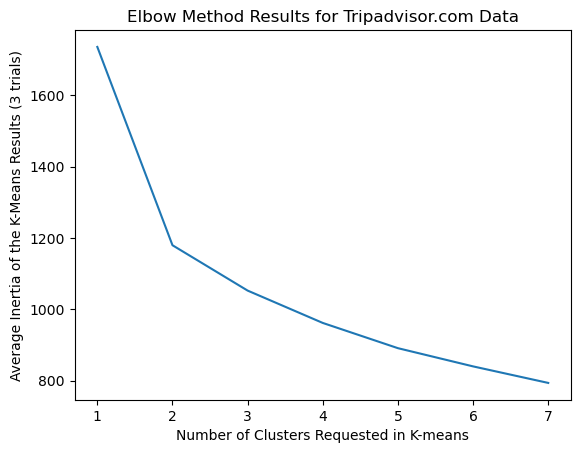
\includegraphics[scale=0.5]{elbow plot.png}
    \caption{Elbow Plot Example}
    \label{}
\end{figure}\end{center}
\subsubsection*{Interpretation of Elbow Plot}
\begin{enumerate}
    \item If there is not a dramatic elbow, then this suggests that either:
    \subitem 1. The dataset is \underline{not clusterable} or
    \subitem 2. K-means is not a suitable algorithm for detecting the underlying clusters.
    \item If there is a dramatic elbow, then this suggests that:
    \subitem 1. There is a clustering structure and
    \subitem 2. The k-means clustering algorithm is suggesting that there are about $K$ clusters where the plot levels off.
\end{enumerate}
In the example of the figure\\
1. We see a somewhat dramatic elbow in the plot. This suggests that there is some clustering structure in the dataset and that k-means is capable of identifying some clustering structure.

2. We see that that plot levels off dramatically at k=2 clusters. So this suggests that asking the k-means algorithm to return k=2 clusters will be the most insightful.

\section{Types of Clusters Definitions}
As we know the K-means algorithm can only work well with data that fulfills specific properties, we define some common \textbf{types of clusters} that could be considered in a numerical dataset to help introduce our new algorithms.

\begin{definition}[Well-Separated Cluster]
    A \textbf{well-separated cluster} defines a cluster only when the data contains natural clusters that are \underline{far apart from each other}. (This definition is vague in how far apart do clusters have to be.)
\end{definition}
Why K-means may not work well?: Well-Separated Cluster can be non-spherical.
\begin{definition}[Density-Based Cluster]
    A \textbf{density-based cluster} defines a cluster as a \underline{dense} region of objects that is surrounded by a region of \underline{lower} density. (This definition is vague in how dense it needs to be considered a cluster.)
\end{definition}
Why K-means may not work well?: Density-Based Cluster can have noise.

\begin{definition}[Graph-Based Cluster]
    \textbf{Graph-based cluster} is a group of objects that are \underline{connected} to one another, but have no \underline{connection} to objects outside the group. (This definition is vague in how do we decide objects are connected.)
\end{definition}
Why K-means may not work well?: Graph-based cluster can be non-spherical and not well separated.

\begin{definition}[Contiguity-Based Cluster (a type of graph-based
    cluster definition)]
    In \textbf{contiguity-based cluster} (a type of graph-based
    cluster definition),  two objects are \underline{connected} only if they are within a \underline{specified distance} of one another.
\end{definition}
\underline{Types of contiguity-based clustering algorithms:} spectral clustering.
\begin{center}\begin{figure}[htbp]
    \centering
    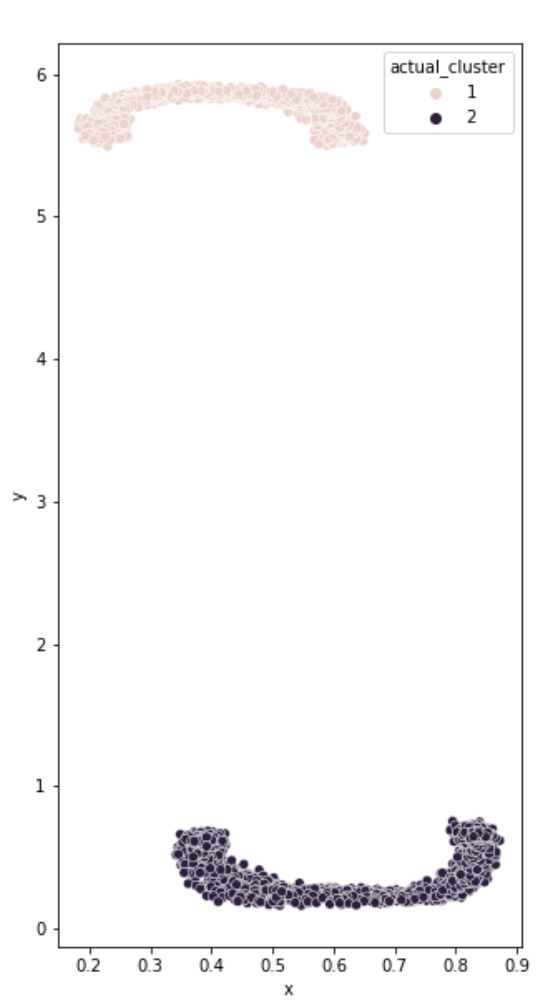
\includegraphics[scale=0.25]{well-separated.png}
    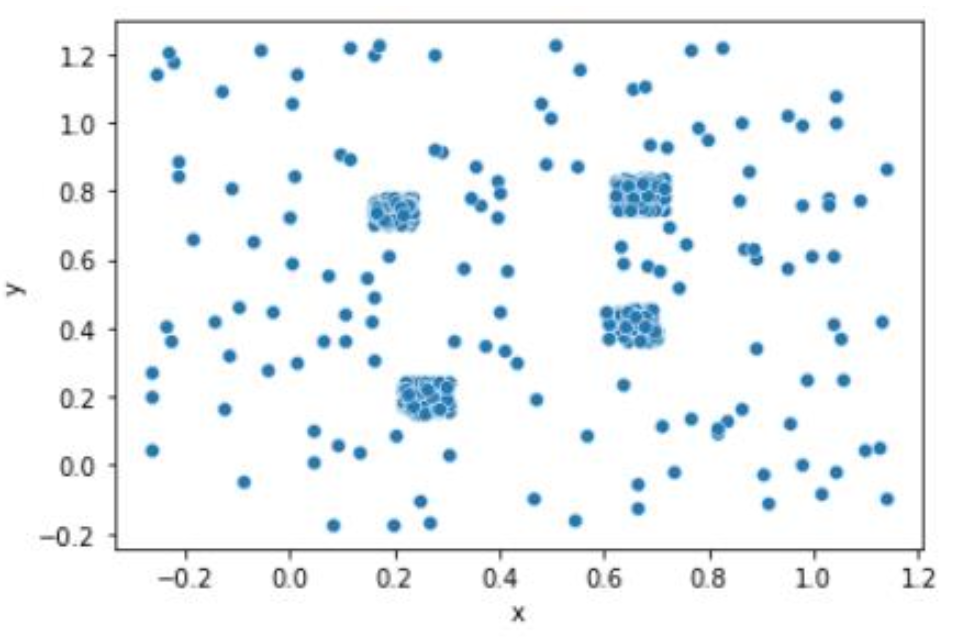
\includegraphics[scale=0.25]{density-based.png}
    \caption{(1). Well-Separated Cluster; (2). Density-Based Cluster}
    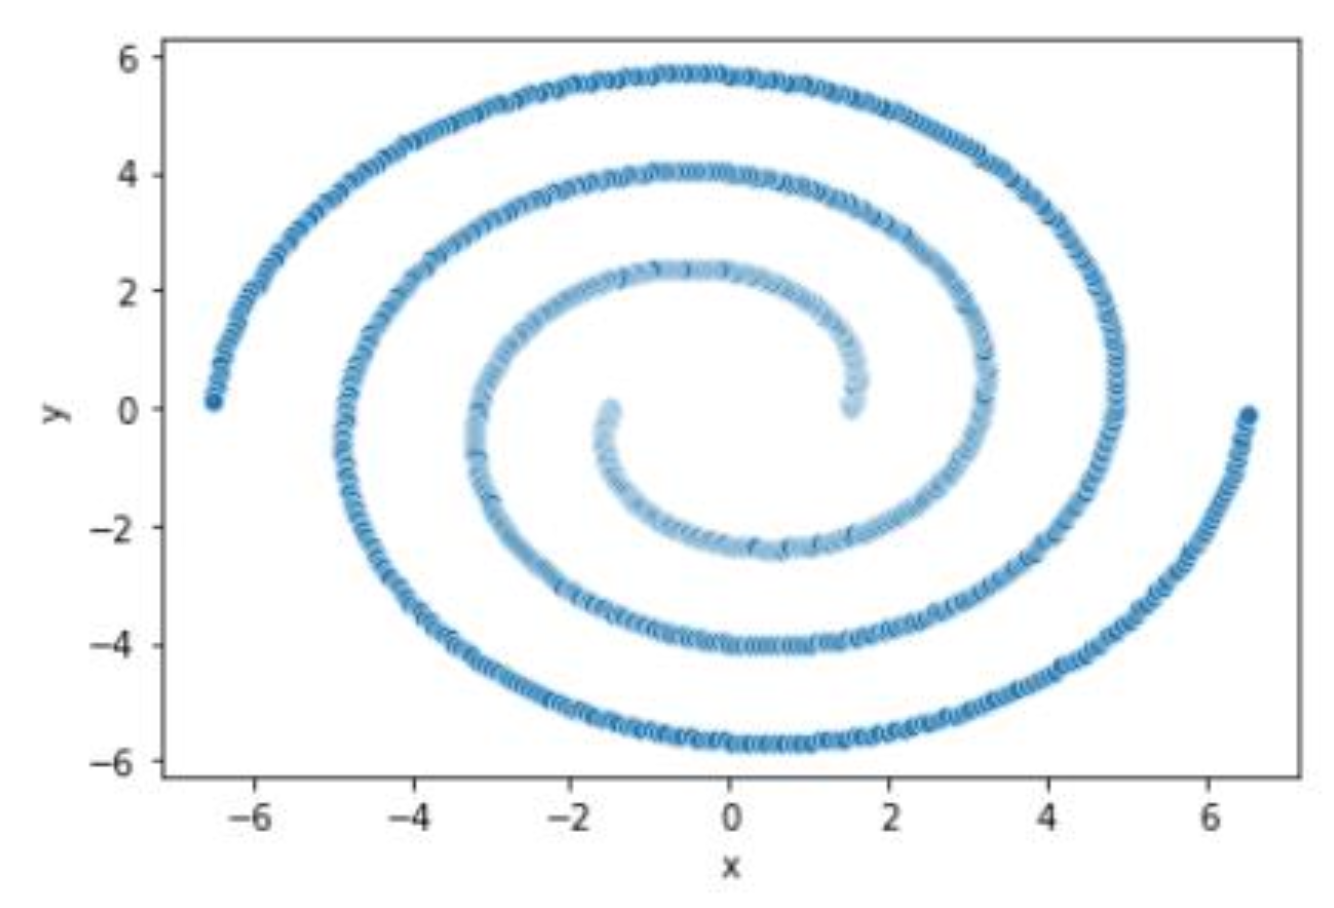
\includegraphics[scale=0.2]{Contiguity-based.png}
    \caption{Contiguity-Based Cluster}
\end{figure}\end{center}

\begin{definition}[Prototype-Based Cluster]
    A \textbf{prototype-based cluster} defines a cluster as a set of objects in which each object is closer (or more similar) to the \underline{prototype} (e.g. mean, median) that defines the cluster than to the \underline{prototype} of any other cluster.
\end{definition}
Why K-means may not work well?: Prototype-Based Cluster may be not well-separated and have outliers.
\begin{center}\begin{figure}[htbp]
    \centering
    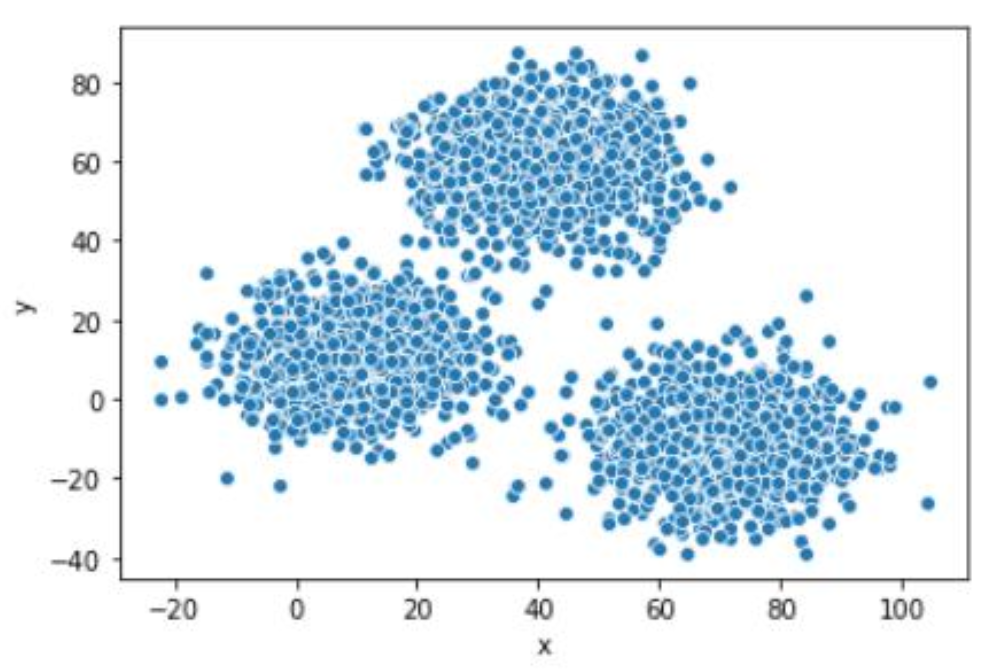
\includegraphics[scale=0.23]{prototype-based.png}
    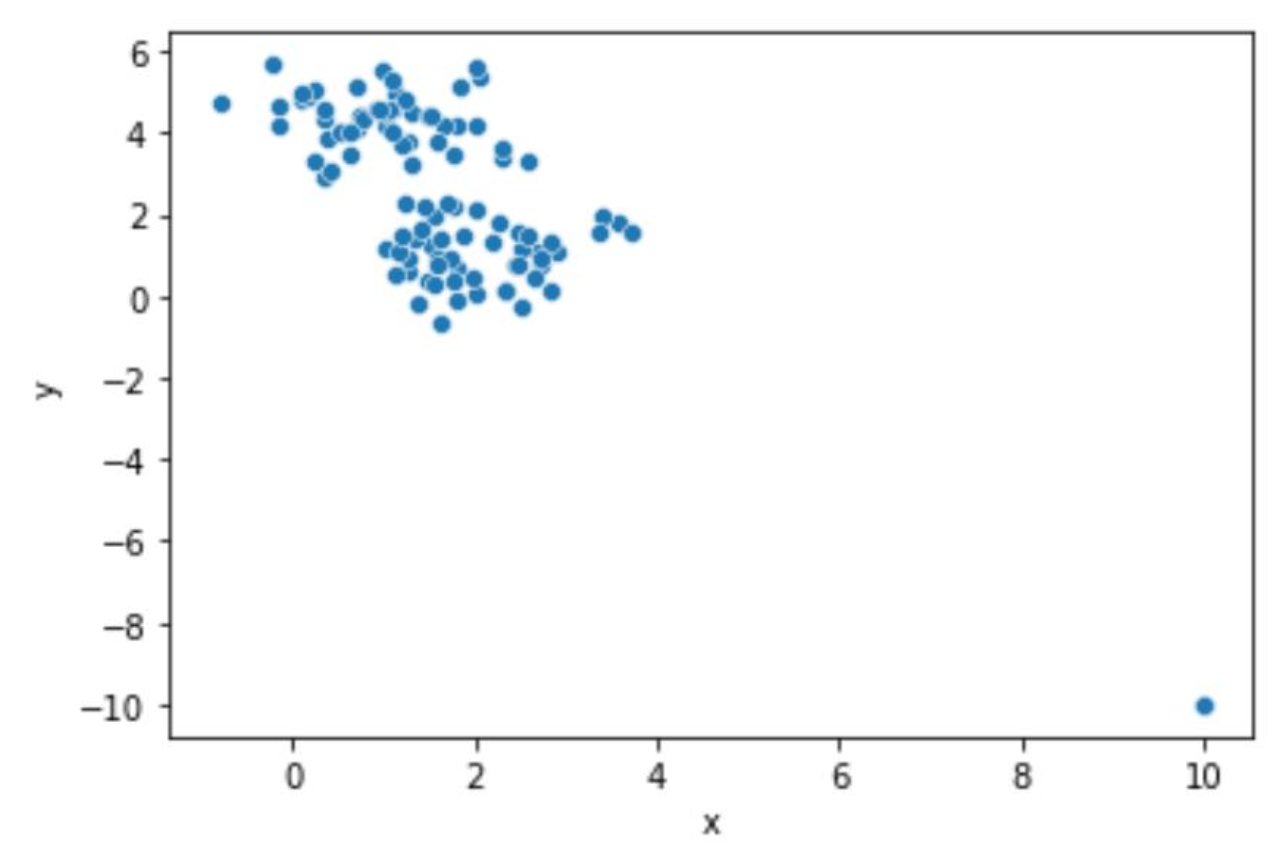
\includegraphics[scale=0.18]{prototype-based2.png}
    \caption{Prototype-Based Cluster}
\end{figure}\end{center}
\underline{Types of prototype-based clustering algorithms:}
\begin{enumerate}[$\bullet$]
    \item \textbf{K-means}: Prototype is the mean of the cluster.
    \item \textbf{K-median}: Prototype is the median of the cluster.
\end{enumerate}


\section{K-Medians}
\subsection{K-Medians Clustering Optimization Problem}

\textbf{Goal of K-Means:}

Out of all possible clustering of $\{S_1 ,S_2 , ... , S_K\}$ with $K$ clusters that can be made from the $m$ objects in $X$, find the optimal clustering $\{S_1^*,S_2^*,...,S_K^*\}$ that \underline{minimizes} the sum of the \underline{Manhattan distances} (i.e., $L_1$ distances) of each object and the centroid (the \underline{median} of the cluster that object is assigned to).

Technically, we can write this as an optimization problem
\begin{equation}
    \begin{aligned}
        \{S_1^*,S_2^*,...,S_K^*\}=\argmin_{S_1,S_2,...,S_K}\sum_{k=1}^K\sum_{x\in S_k}\|x-c_k\|_1\\
        \textnormal{Optimal Inertia}=\min_{S_1,S_2,...,S_K}\sum_{k=1}^K\sum_{x\in S_k}\|x-c_k\|_1\\
    \end{aligned}
    \nonumber
\end{equation}

\subsection{K-Medians Heuristic Algorithm}
\begin{enumerate}
    \item \textbf{Input:}
    \subitem Desired number of clusters (ex: $K=3$)
    \subitem Dataset of $m$ objects $X=\{\vec{x}_1,\vec{x}_2,...,\vec{x}_m\}$, where each object $\vec{x}_i=(x_{i1},x_{i2},...x_{in})$ has $n$ numerical attributes. (We can also think of $X$ as being an $m\times n$ matrix $X_{m\times n}$.)
    \item \textbf{Algorithm:}
    \begin{enumerate}[$\bullet$]
        \item \textbf{\underline{Step 1:} Centroid Initialization Step}\\
        Randomly select $K$ centroids $\{\vec{c}_1,\vec{c}_2,...,\vec{c}_K\}$, where $\vec{c}_k=(c_{k1},c_{k2},...,c_{kn})$
        \item \textbf{\underline{Step 2:} Cluster Assignment Step}\\
        Assign each object $x_i$ in the dataset to its \underline{closest} centroid (specifically the \textit{smallest Manhattan distance})
        \item \textbf{\underline{Step 3:} Centroid Update Step}\\
        Find the \underline{median} of each cluster created in step 2. These medians are now the new \underline{centroids}.
        \item \textbf{\underline{Step 4:} Stopping Criterion}\\
        If the old centroids and the new centroids are the \underline{same}, stop the algorithm. Otherwise, go back to step 2.
    \end{enumerate}
    \item \textbf{Output:} Clustering with $K$ clusters $\{V_1,V_2,...,V_K\}$.
\end{enumerate}


\section{K-Medoids}
\begin{definition}[Medoid]
    In the context of clustering, we define a \textbf{medoid} as \underline{an actual object} in a cluster whose sum of distance to all the objects in the cluster is minimal.
\end{definition}
\subsection{K-Medoids Clustering Optimization Problem}

\textbf{Goal of K-Medoids:}

Out of all possible clustering of $\{S_1 ,S_2 , ... , S_K\}$ with $K$ clusters that can be made from the $m$ objects in $X$, find the optimal clustering $\{S_1^*,S_2^*,...,S_K^*\}$ that \underline{minimizes} the sum of the \underline{distances} (any distance metric) of each object and the centroid (the \underline{medoid} of the cluster that object is assigned to).

Technically, we can write this as an optimization problem
\begin{equation}
    \begin{aligned}
        \{S_1^*,S_2^*,...,S_K^*\}=\argmin_{S_1,S_2,...,S_K}\sum_{k=1}^K\sum_{x\in S_k}\textnormal{dist}(x,c_k)\\
        \textnormal{Optimal Inertia}=\min_{S_1,S_2,...,S_K}\sum_{k=1}^K\sum_{x\in S_k}\textnormal{dist}(x,c_k)\\
    \end{aligned}
    \nonumber
\end{equation}

\subsection{K-Medoids Clustering Algorithm}
\begin{enumerate}
    \item \textbf{Input:}
    \subitem Desired number of clusters (ex: $K=3$)
    \subitem Dataset of $m$ objects $X=\{\vec{x}_1,\vec{x}_2,...,\vec{x}_m\}$, where each object $\vec{x}_i=(x_{i1},x_{i2},...x_{in})$ has $n$ numerical attributes. (We can also think of $X$ as being an $m\times n$ matrix $X_{m\times n}$.)
    \item \textbf{Algorithm:}
    \begin{enumerate}[$\bullet$]
        \item \textbf{\underline{Step 1:} Centroid Initialization Step}\\
        Randomly select $K$ centroids $\{\vec{c}_1,\vec{c}_2,...,\vec{c}_K\}$, where $\vec{c}_k=(c_{k1},c_{k2},...,c_{kn})$
        \item \textbf{\underline{Step 2:} Cluster Assignment Step}\\
        Assign each object $x_i$ in the dataset to its \underline{closest} centroid (specifically the \textit{using distance metric you've chosen})
        \item \textbf{\underline{Step 3:} Centroid Update Step}\\
        Find the \underline{medoid} of each cluster created in step 2. These medians are now the new \underline{centroids}.
        \item \textbf{\underline{Step 4:} Stopping Criterion}\\
        If the old centroids and the new centroids are the \underline{same}, stop the algorithm. Otherwise, go back to step 2.
    \end{enumerate}
    \item \textbf{Output:} Clustering with $K$ clusters $\{V_1,V_2,...,V_K\}$.
\end{enumerate}

\subsection{K-Medoids vs. K-Means}
\subsubsection*{Benefit of K-Medoids over K-Means:}
\begin{enumerate}
    \item The medoid is more robust to outliers.
    \item Guaranteed to converge using any distance metric we want (K-means has to use squared euclidean distance).
\end{enumerate}
\subsubsection*{Benefit of K-Means over K-Medoids:}
K-Medoids is more computationally complex than k-means:
\begin{enumerate}
    \item K-means: $O\left(\textnormal{number of objects}\times \textnormal{number of attributes}\times \textnormal{number of clusters}\times \textnormal{number of iterations}\right)$
    \item K-medoids: $O\left((\textnormal{number of objects})^2\times \textnormal{number of attributes}\times \textnormal{number of clusters}\times \textnormal{number of iterations}\right)$
\end{enumerate}

\section{Types of Clustering Algorithms Results}
\subsection{Partitional vs. Hierarchical Clustering Results}
\begin{definition}[Partitional Clustering]
    We call a \textbf{partitional clustering} a division of the set of data objects into $k$ subsets (clusters) such that each object is in \underline{exactly one} subset.
\end{definition}
\begin{example}
    $\{1,2,8\},\{3,7\},\{4,5,6\}$
\end{example}

\begin{definition}[Hierarchical Clustering]
    In a \textbf{hierarchical clustering} we allow for clusters to have \underline{nested subclusters}.\\
    A hierarchical
    clustering is displayed as a set of nested clusters displayed as a \textbf{dendrogram} tree. The dendrogram can reflect which objects and clusters are closer to each other than others.
\end{definition}
\begin{example}
    $\{\{1,3\},\{\{\{6,9\},10\},\{11,15\}\}\},\{4,\{12,19\}\},\{\{\{2,14\},\{\{17,20\},18\}\},\{5,8\}\},\{7,\{13,16\}\}$.
\end{example}
\begin{center}\begin{figure}[htbp]
    \centering
    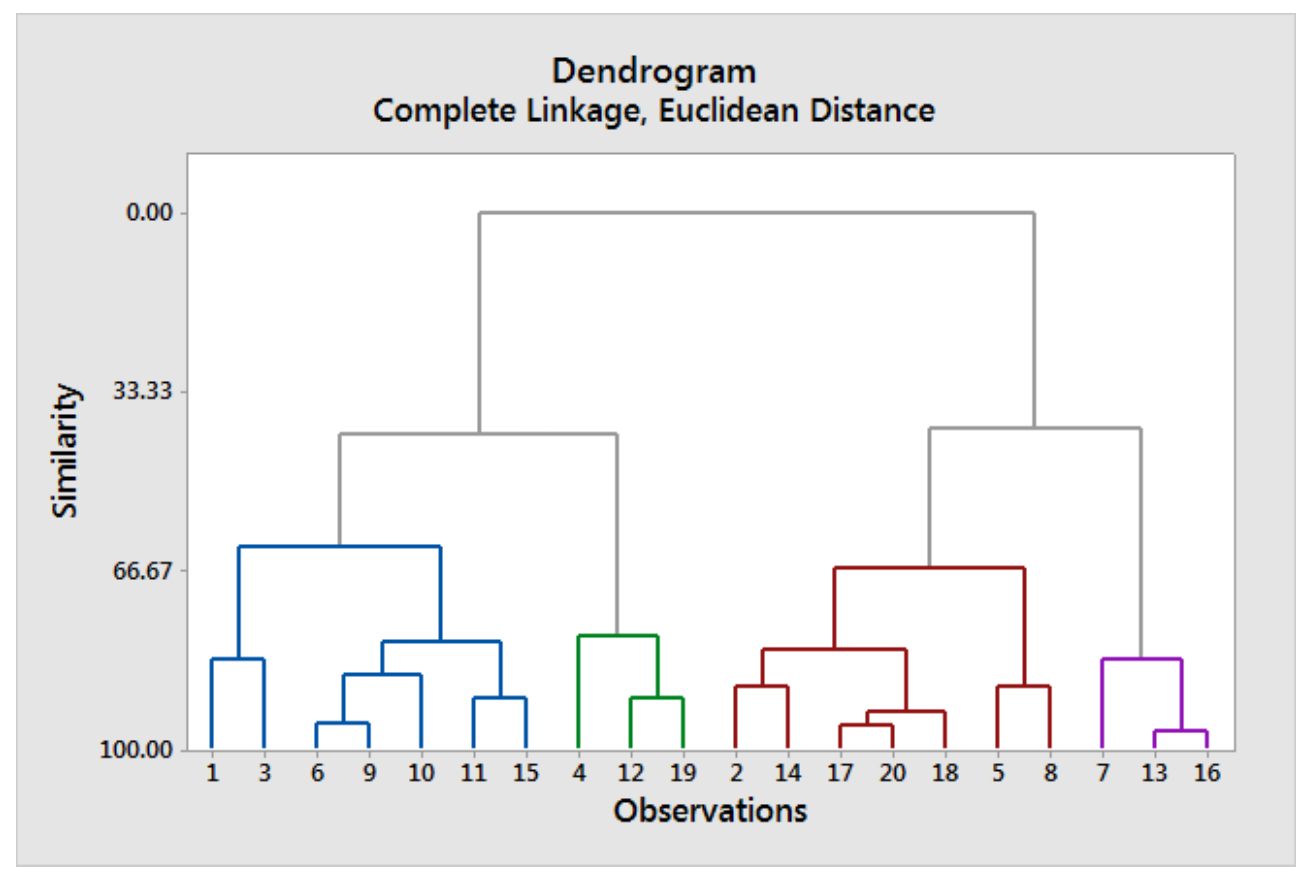
\includegraphics[scale=0.25]{Hierarchical Clustering.png}
    \caption{Hierarchical Clustering Example}
    \label{}
\end{figure}\end{center}

\subsection{Exclusive vs. Overlapping vs. Fuzzy Clustering Results}
\begin{definition}
    \textbf{Exclusive Clustering} will assign an object to an \underline{exactly one cluster}.
\end{definition}
\begin{example}
    $\{1,3,5\},\{2,4\}$.
\end{example}
\begin{definition}
    \textbf{Overlapping Clustering} can allow for an object to be assigned to \underline{more than one cluster}.
\end{definition}
\begin{example}
    $\{1,3,5\},\{2,4,5\}$
\end{example}

\begin{definition}
    In a \textbf{Fuzzy Clustering} every object belongs to every cluster with a membership weight that is between $0$ (absolutely doesn't belong to the cluster) to $1$ (absolutely belongs).
    \begin{enumerate}
        \item Usually the sum of each object's weights must sum to $1$.
        \item $w_{ij}$ $=$ the probability that object $i$ belongs to cluster $j$.
    \end{enumerate}
\end{definition}








\chapter{Clustering Evaluation Metrics}
\section{Clusterability Evaluation Metric: Is the dataset clusterable?}
\begin{definition}
    A dataset is \textbf{clusterable} if there exist some distinct groupings of observations in a dataset.
\end{definition}
Then, how distinct do the observation need to be is a question.


\subsection{Hopkin's Statistics}
\begin{enumerate}[$\bullet$]
    \item \textbf{\underline{Input:}} Dataset of $m$ objects $X=\{\vec{x}_1,\vec{x}_2,...,\vec{x}_m\}$, where each object $\vec{x}_i=(x_{i1},x_{i2},...x_{in})$ has $n$ numerical attributes.
    \item \textbf{\underline{How to calculate:}}
    \begin{enumerate}[$(1)$]
        \item Create a set of random \underline{artificial data point} closest distances $\{u_1,u_2,...,u_p\}$ as follows.
        \begin{enumerate}[a)]
            \item Generate $p$ \underline{random artificial data points} $\{\vec{y}_1, \vec{y}_2, ... , \vec{y}_p\}$ distributed across
            the range of the dataset.
            \item For each random artificial data points $i=1,...,p$ calculate $$u_i=\min_{\vec{x}\in X}\textnormal{dist}(\vec{y}_i,\vec{x})$$
        \end{enumerate}
        \item Create a set of random \underline{actual data point} closest distances $\{w_1,w_2,...,w_p\}$ as follows.
        \begin{enumerate}[a)]
            \item Random select $p$ \underline{actual points} $\{\vec{z}_1, \vec{z}_2, ... , \vec{z}_p\}$ from the dataset.
            \item For each randomly selected actual points $i=1,...,p$ calculate $$w_i=\min_{\vec{x}\in X}\textnormal{dist}(\vec{z}_i,\vec{x})$$
        \end{enumerate}
        \item $$\textbf{Hopkins Statistic}=\frac{\sum_{i=1}^p w_i}{\sum_{i=1}^p w_i+\sum_{i=1}^p u_i}$$
    \end{enumerate}
    \item \textbf{\underline{How to interpret:}} The dataset is \underline{clusterable} if the Hopkins Statistic \underline{close to $0$} and is \underline{not clusterable} if the Hopkins Statistic \underline{close to $0.5$}.
    \item \textbf{\underline{Intuition:}}
    \begin{center}\begin{figure}[htbp]
        \centering
        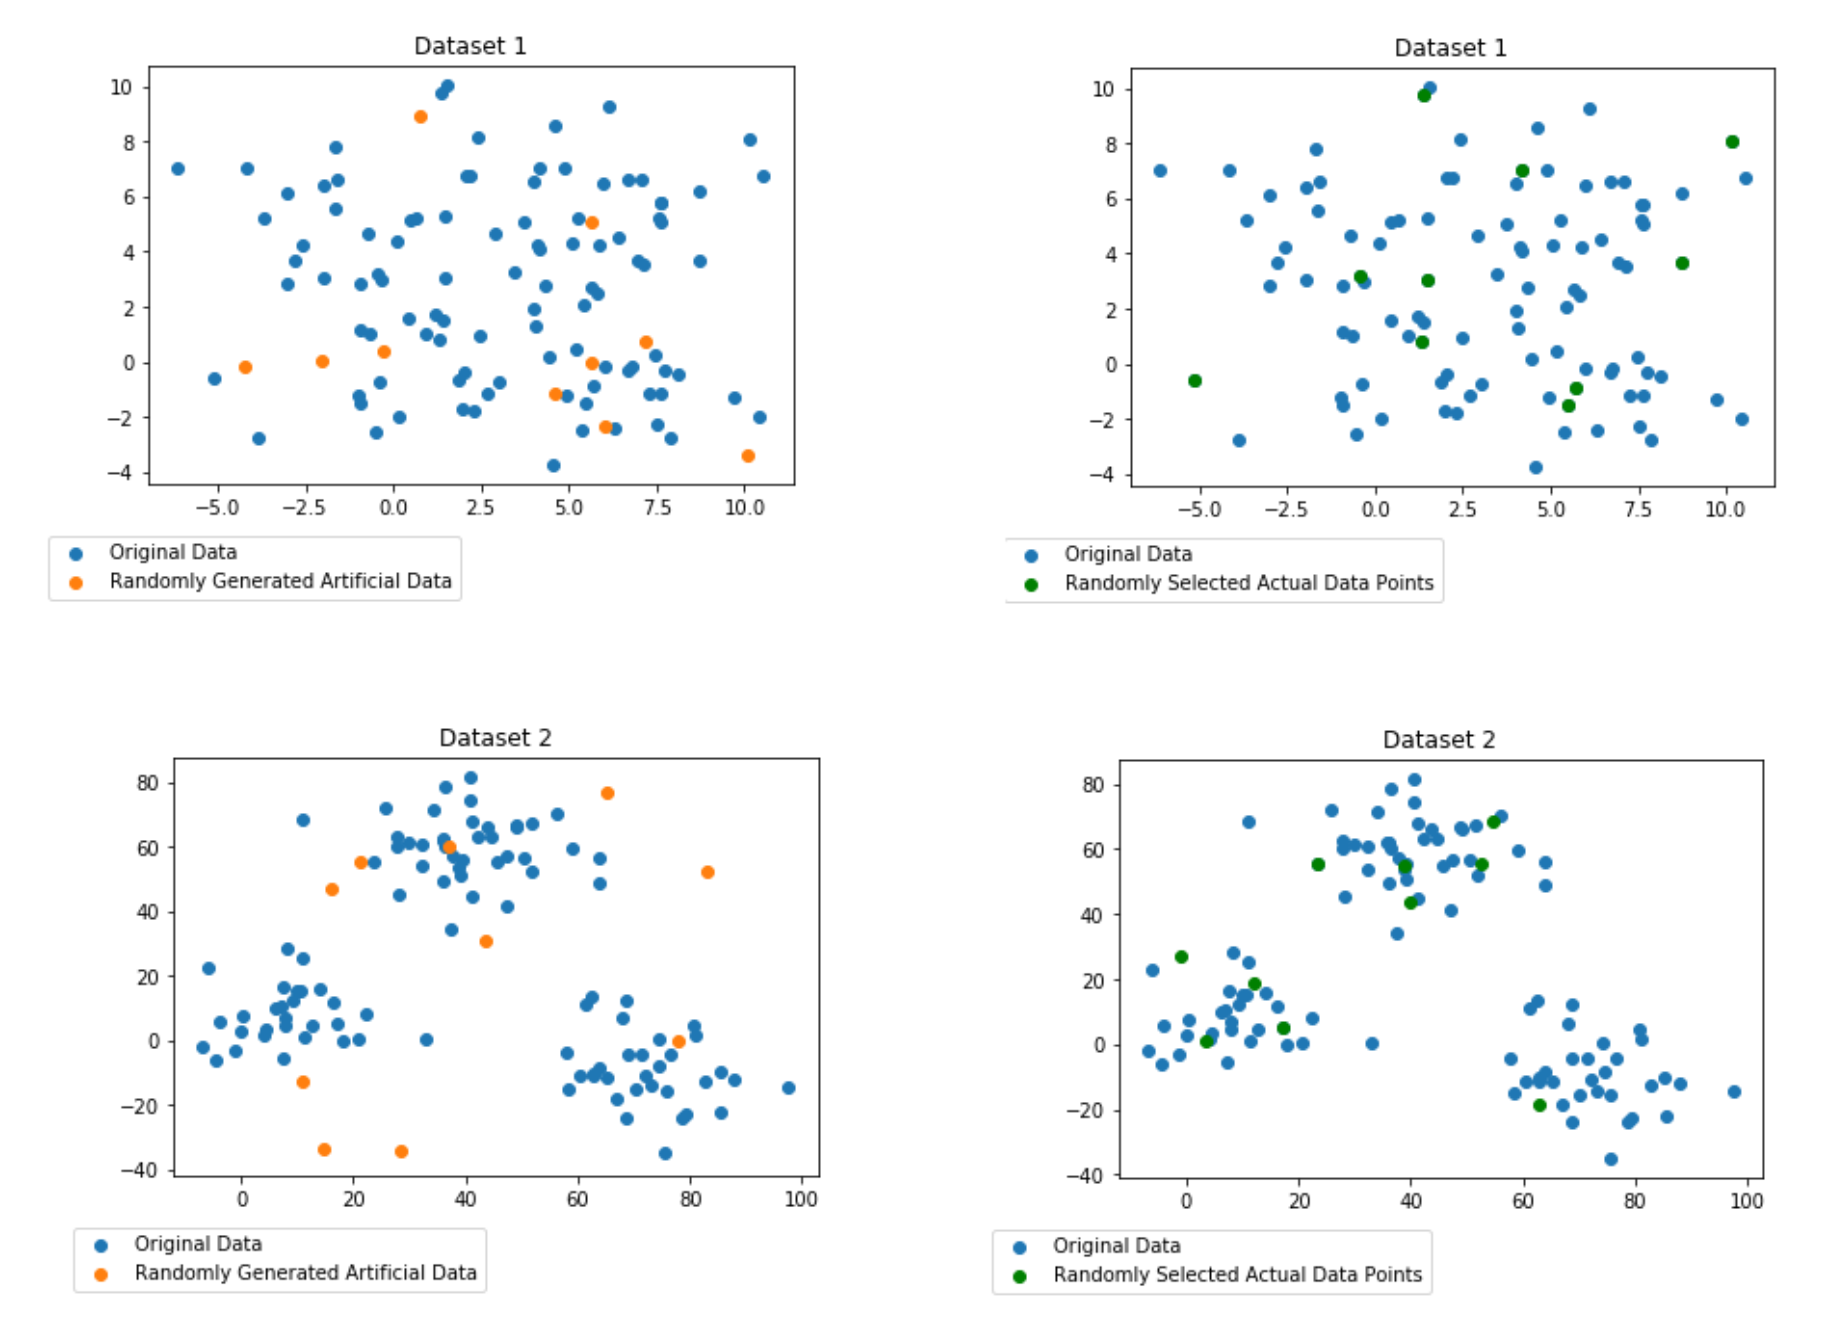
\includegraphics[scale=0.25]{HS.png}
        \caption{When Hopkins Statistic works well and not well}
        \label{}
    \end{figure}\end{center}
    \item \textbf{\underline{Additional Tips and Information:}} $p=10\%\times \textnormal{(the number of observations in the dataset)}$; Hopkins Statistic is \underline{non-deterministic} evaluation metric.
\end{enumerate}

\section{Unsupervised Clustering Evaluation Metrics: How cohesive and well separated are the clusters in the
clustering?}
\subsection{Definition}
\begin{definition}
    \textbf{Unsupervised clustering evaluation metrics} evaluate the goodness of the clustering without using pre-assigned class labels.
\end{definition}

\underline{Types of Unsupervised Clustering Evaluation Metrics:}
\begin{enumerate}
    \item \textbf{Cohesion} measures how closely related the objects in a cluster are.
    \item \textbf{Separation} measures how distinct or well-separated a cluster is from other clusters.
    \item \textbf{Validity of a clustering} can be expressed as some function of \textbf{cohesion} and \textbf{separation} of all the clusters in a clustering.
\end{enumerate}

\subsection{Graph-based view of cohesion and separation for a clustering}
A graph-based view of calculating cohesion and separation for a clustering involves first creating a \textbf{proximity matrix} (graph) of the objects in the dataset, that measures the “proximity” of each pair of objects in the dataset.
\begin{center}\begin{figure}[htbp]
    \centering
    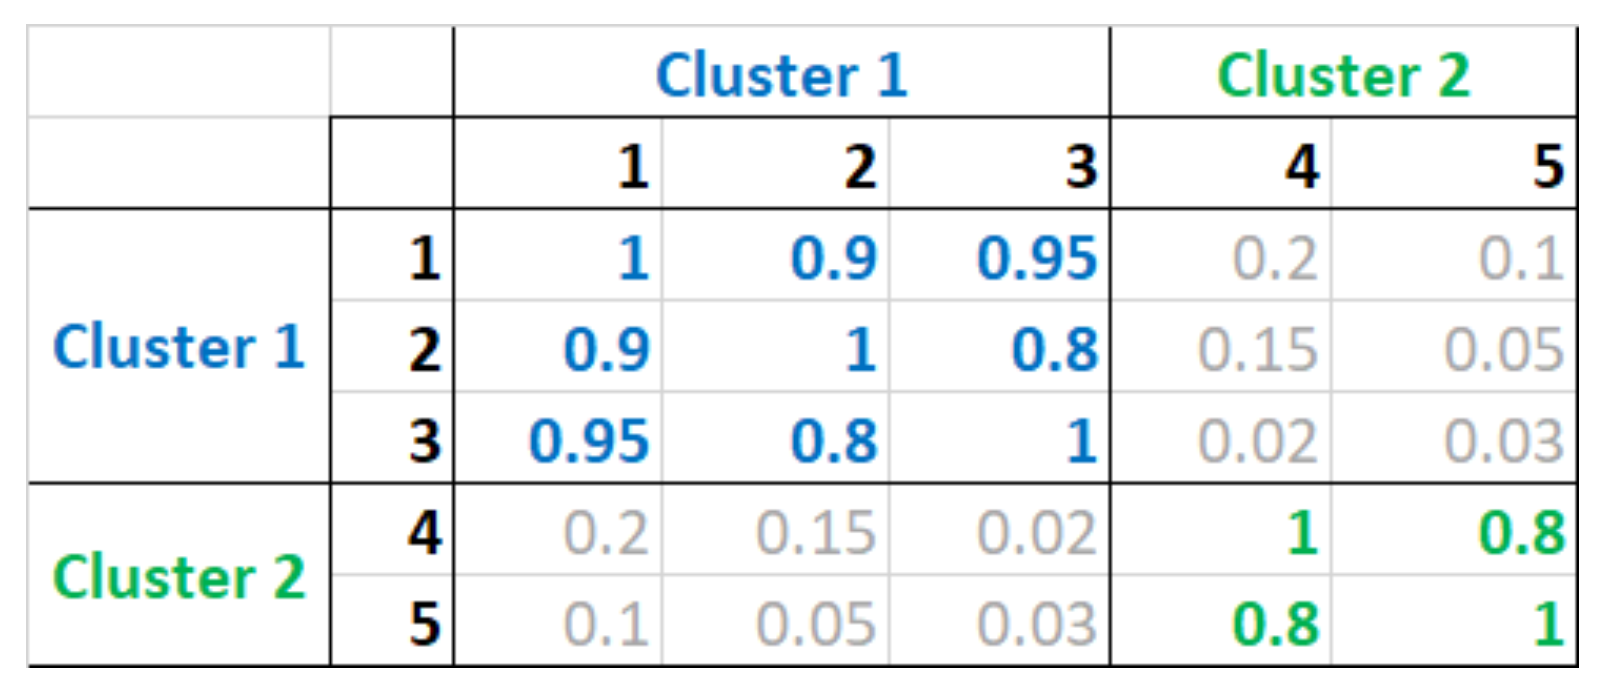
\includegraphics[scale=0.18]{proximity matrix.png}
    \caption{Proximity Matrix}
    \label{}
\end{figure}\end{center}
\underline{Different ways to measure proximity:}
\begin{enumerate}
    \item \textbf{Similarity metric measure of proximity:} The more similar two objects are the lower the proximity measure is. e.g. Euclidean distance.
    \item \textbf{Dissimilarity metric measure of proximity:} The more similar two objects are the higher this proximity measure is. e.g. The number of attribute agreements between two categorical objects.
\end{enumerate}

\underline{\textbf{Cohesion} of a graph-based cluster} is the sum of proximities between all pairs of points within the same cluster.
\begin{equation}
    \begin{aligned}
        \textnormal{cohesion}(C_i)=\sum_{\vec{x}\in C_i,\vec{y}\in C_i}\textnormal{proximity}(\vec{x},\vec{y})
    \end{aligned}
    \nonumber
\end{equation}

\underline{\textbf{Separation} of a graph-based cluster} is the sum of proximities between all pairs of points in the two different clusters.
\begin{equation}
    \begin{aligned}
        \textnormal{separation}(C_i,C_j)=\sum_{\vec{x}\in C_i,\vec{y}\in C_j}\textnormal{proximity}(\vec{x},\vec{y})
    \end{aligned}
    \nonumber
\end{equation}

\subsection{Silhouette Coefficients (Scores)}
\begin{enumerate}
    \item \textbf{Cohesion Metric:} Measure of how “well assigned” object $x_i$ is to cluster $C_k$: $$a_i=\frac{1}{|C_k|-1}\sum_{\vec{x}_j\in C_k,\vec{x}_i\neq \vec{x}_j}\textnormal{dist}(\vec{x}_i,\vec{x}_j)$$
    \item \textbf{Separation Metric:} Find the Average Distance of object $x_i$ to it's "neighboring cluster." $$b_i=\min_{k'\neq k}\frac{1}{|C_{k'}|}\sum_{\vec{x}_j\in C_{k'}}\textnormal{dist}(\vec{x}_i,\vec{x}_j)$$
    \item \textbf{Silhouette Coefficient (Score)} of $x_i$
    $$s_i=\left\{\begin{matrix}
        \frac{b_i-a_i}{\max\{a_i,b_i\}},&\textnormal{if }|C_i|>1\\
        0,&\textnormal{if }|C_i|=1
    \end{matrix}\right.$$
\end{enumerate}
The silhouette of a cluster visualizes the silhouette values $s_i$ of all the points in it in the \underline{decreasing order}. A silhouette plot shows the silhouettes of all the clusters in random order. Additionally, it inserts blank spaces between consecutive clusters and can color them differently.
\begin{center}\begin{figure}[htbp]
    \centering
    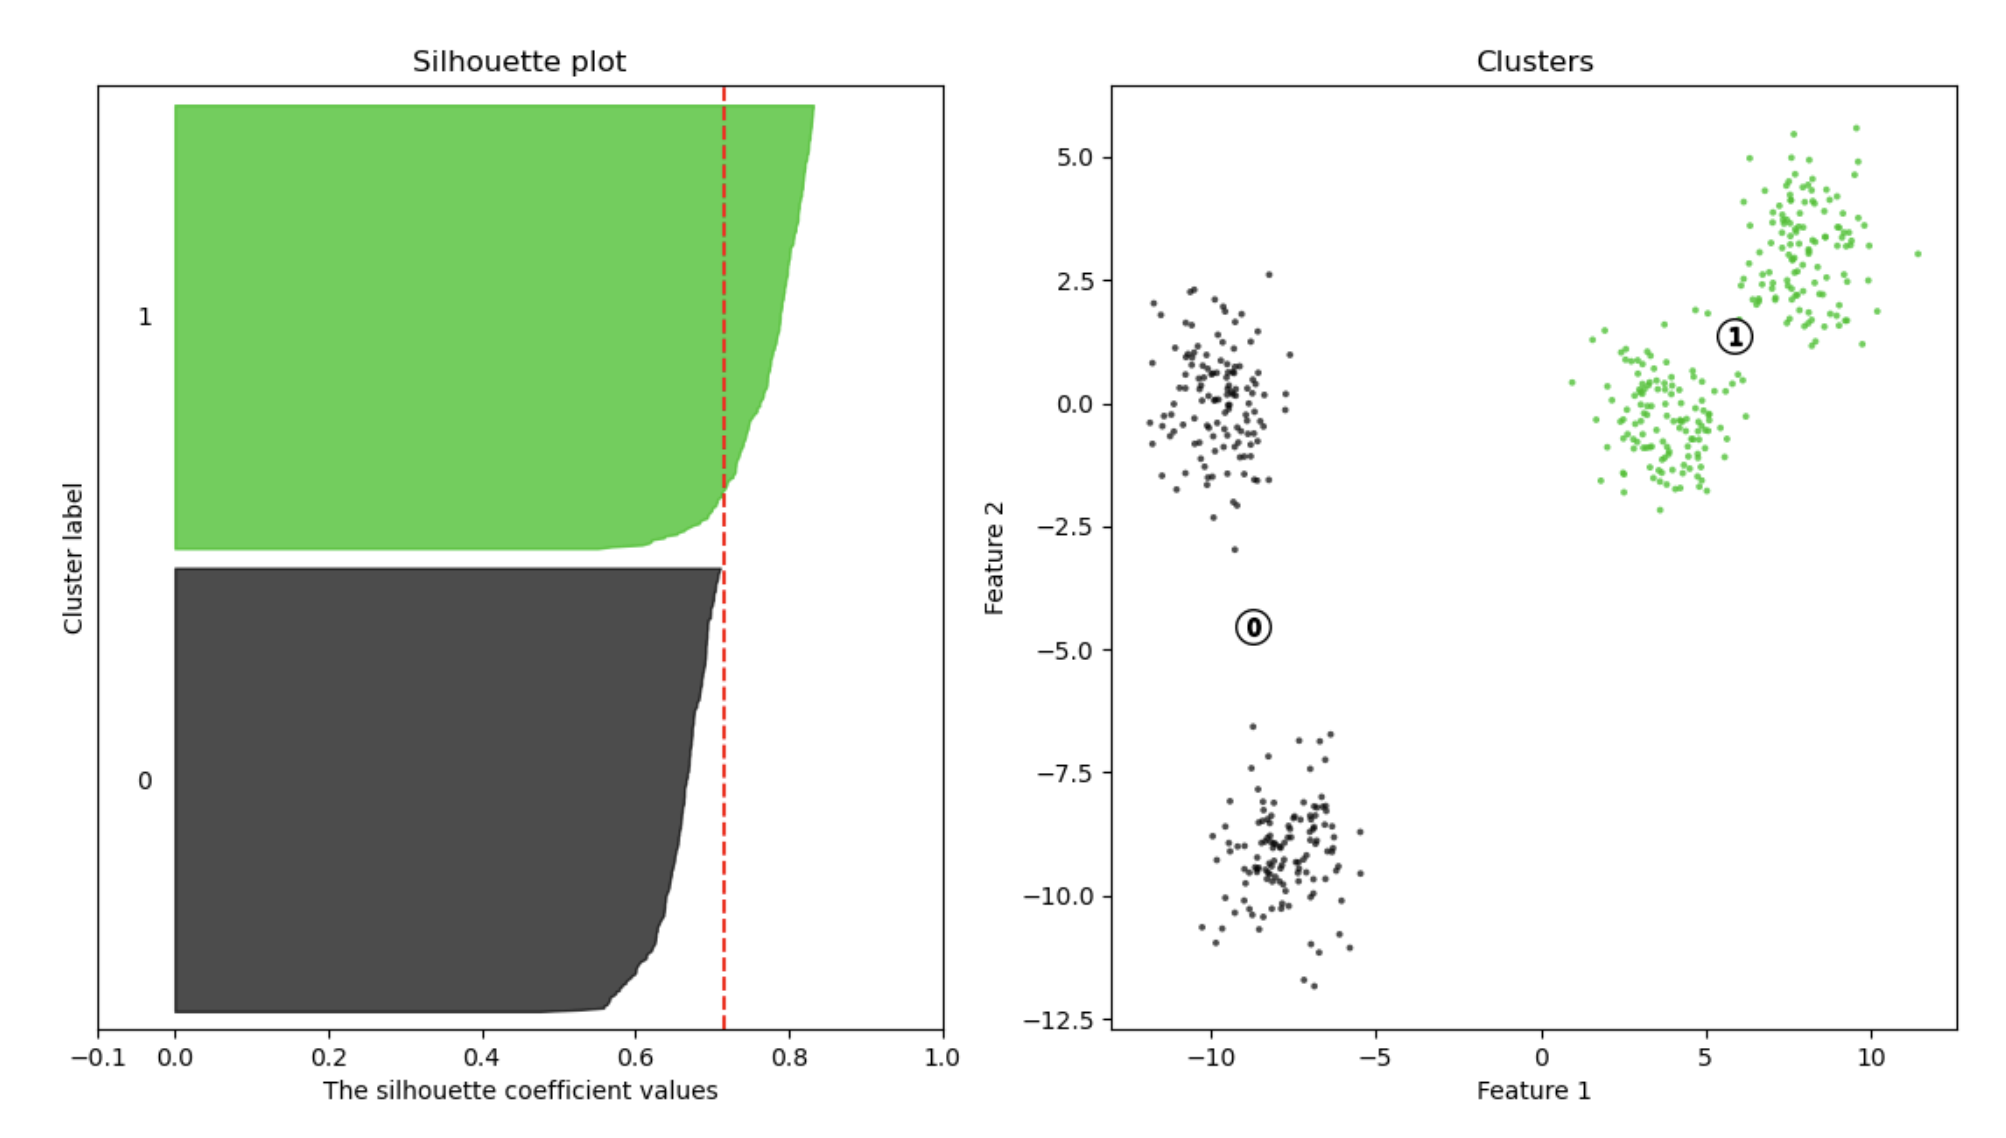
\includegraphics[scale=0.2]{Silhouette Plots.png}
    \caption{Silhouette Plots}
    \label{}
\end{figure}\end{center}

\begin{enumerate}
    \item \textbf{Silhouette Coefficient} $s_i$ of object $\vec{x}_i$ is \underline{large and positive}: the object is \underline{closer} to objects in the cluster that it is assigned to than objects in other clusters.
    \item \textbf{Silhouette Coefficient} $s_i$ of object $\vec{x}_i$ is \underline{close to $0$}: the object is \underline{equally close} to objects in the cluster that it is assigned to than objects in other clusters.
    \item \textbf{Silhouette Coefficient} $s_i$ of object $\vec{x}_i$ is \underline{large and negative}: the object is \underline{further away from} to objects in the cluster that it is assigned to than objects in other clusters.
\end{enumerate}
\textbf{Warning:} Silhouette coefficients and plots (based off of Euclidean distances) will not be effective at assessing clustering separation and cohesion for all types of datasets. (e.g. the contiguity-based cluster.) We need to revise the distance metric.

\subsection{Prototype-Based View of Cohesion and Separation for a Clustering}
\begin{enumerate}
    \item \textbf{Cohesion of a prototype-based cluster:} the sum of proximities between all points \underline{in a given cluster} and the \underline{prototype} of that cluster.
    \item \textbf{Separation of a prototype-based cluster:} the proximity of the two cluster prototypes.
\end{enumerate}


\section{Cluster Number Evaluation Metrics: What is the 'correct' number of clusters?}

\subsection{General Elbow Plot Method}
\begin{definition}[General Elbow Plot Method]
    When determining whether a clustering structure can be detected by a particular clustering algorithm (K-means, K-medians, K-medoids), we can use an elbow plot that plots the value of the objective function that we are trying to minimize of the clusterings found by that particular clustering algorithm with $k=1,k=2,...$ clusters respectively.
\end{definition}

The \textbf{drawback} of this method is each of these methods are dependent on the ability of a clustering algorithm to detect the clustering structure.

\subsection{Average Silhouette Score Plot Method}
\begin{enumerate}[(1).]
    \item \textbf{\underline{Creating an Average Silhouette Score Plot}}\\
    For $k=1$ to $K$:
    \begin{enumerate}[$\bullet$]
        \item Cluster the data several times into k clusters.
        \item Calculate the average of the average silhouette scores of these resulting
        clusterings.
        \item Then plot the average of these average silhouette scores for each $k$.
    \end{enumerate}
    \begin{center}\begin{figure}[htbp]
        \centering
        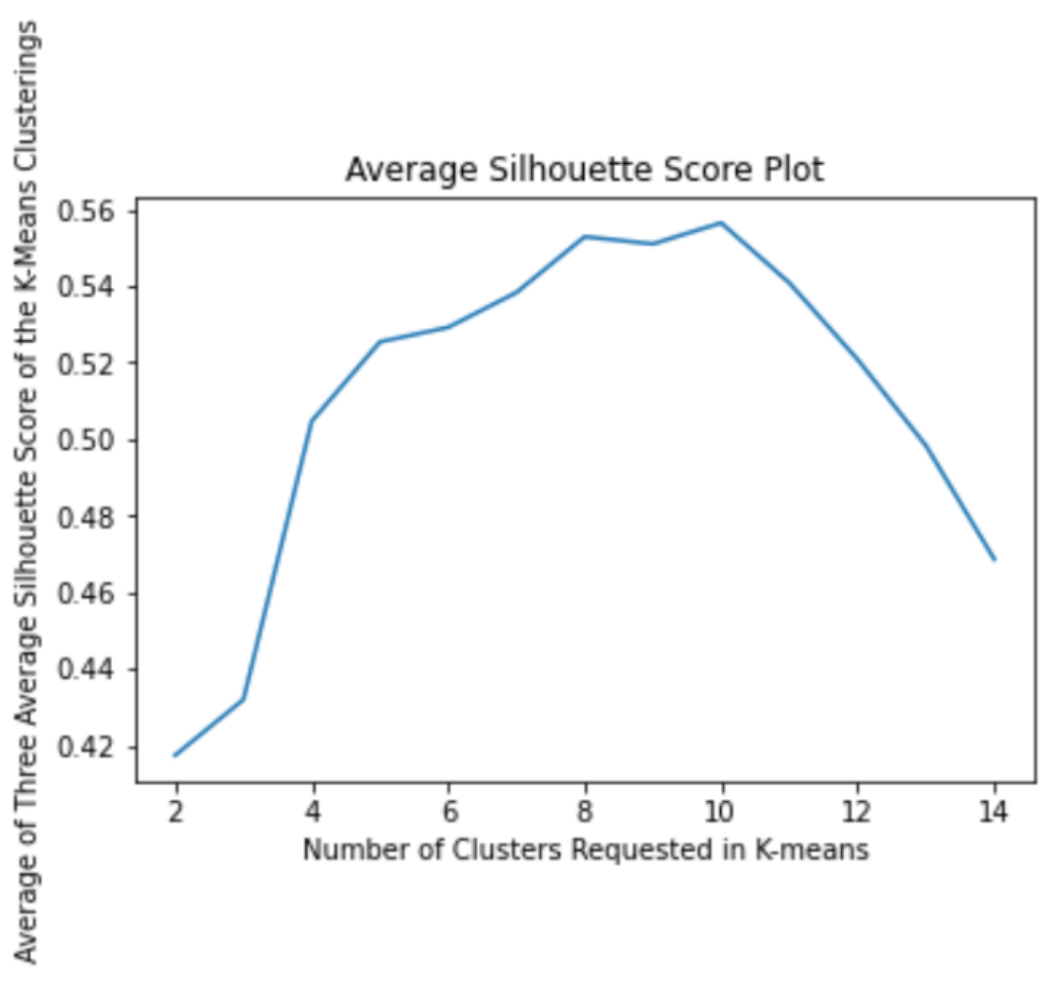
\includegraphics[scale=0.2]{Average Silhouette Score Plot.png}
        \caption{Average Silhouette Score Plot}
        \label{}
    \end{figure}\end{center}
    \item \textbf{\underline{How to interpret:}} Choose the number of clusters with the highest average silhouette score.
    \item \textbf{\underline{Warning:}} We need to make sure the distance metric we are using to measure the silhouette score with is a useful metric in measuring the cohesion and the separation of
    the clusters in the dataset.\\
    For instance, when using the Euclidean distance to measure distance in the silhouette score, the average silhouette score is not as effective in measuring clustering cohesion and separation of \textbf{non-convex shapes}.
    \item \textbf{\underline{Benefit:}} Using an average silhouette score plot do not assume using one particular algorithm/clustering problem to measure cluster performance.
\end{enumerate}




\section{Supervised Clustering Evaluation Metrics: How similar is the clustering to a set of (external) pre-assigned class labels?}

\begin{definition}[Supervised Clustering Evaluation Metrics]
    \textbf{Supervised clustering evaluation metrics} evaluate the clustering by using a set of pre-assigned class labels. This can be useful for examining the association between our pre-assigned cluster labels and the clustering structure identified by our clustering algorithms.
\end{definition}

\subsection{Rand Index and Jaccard Coefficient of Two Partitions}
A partition of a set $\{x_1, x_2, ... , x_m\}$ is a collection of $K$ non-empty subsets (i.e. clusters/classes) of the set such that every element of the set is in exactly one of the subsets (i.e. clusters/classes).
\begin{definition}[Rand Index and Jaccard Coefficient]
    \begin{equation}
        \begin{aligned}
            \textnormal{Rand Index (Statistic)}&=\frac{f_{00}+f_{11}}{f_{00}+f_{01}+f_{10}+f_{11}}\\
            \textnormal{Jaccard Coefficient}&=\frac{f_{11}}{f_{01}+f_{10}+f_{11}}\\
        \end{aligned}
        \nonumber
    \end{equation}
    \begin{enumerate}[$\circ$]
        \item $f_{00}=$ number of pairs of objects in the dataset that are \textbf{apart} in partition 1 and partition 2
        \item $f_{11}=$ number of pairs of objects in the dataset that are \textbf{together} in partition 1 and partition 2
        \item $f_{01}=$ number of pairs of objects in the dataset that are \textbf{apart} in partition 1 and \textbf{together} in partition 2
        \item $f_{10}=$ number of pairs of objects in the dataset that are \textbf{together} in partition 1 and \textbf{apart} in partition 2
    \end{enumerate}
\end{definition}
\textbf{Interpretation and Ranges:}
\begin{enumerate}
    \item Rand Index (Statistic)$\in [0,1]$: $0$ means all possible object pairs disagree between the two partitions; $1$ means the partitions are exactly the same.
    \item Jaccard Coefficient$\in [0,1]$: $0$ means none of the possible object pairs that have
    at least one partition
    that has put them
    together are together in both partitions; $1$ means all possible object pairs that have at least one partition that has put them together are together in both partitions.
\end{enumerate}

\subsection{Adjusted Rand Index}
In Rand Index (Statistic), $0$ means all possible object pairs disagree between the two partitions and $1$ means clusterings are identical. However, we want a desired evaluation metric such that, $0$ means random labeling independently of the number of clusters and samples and $1$ means clusterings are identical

\begin{definition}[Adjusted Rand Index]
    \begin{equation}
        \begin{aligned}
            \textnormal{Adjusted Rand Index}=\frac{\textnormal{rand index}-\textnormal{expected rand index}}{\textnormal{maximum rand index}-\textnormal{expected rand index}}
        \end{aligned}
        \nonumber
    \end{equation}
\end{definition}
For two partitions $\{U_1,U_2,...,U_K\}$ and $\{V_1,V_2,...,V_{K'}\}$ of the same set of $m$ objects, we can define:
\begin{enumerate}
    \item $m_{k,k'}=$number of objects in common in subset $U_k$ and $V_{k'}$.
    \item $a_k=$the total number objects in subset $U_k$.
    \item $b_{k'}=$the total number objects in subset $V_{k'}$.
\end{enumerate}
\begin{equation}
    \begin{aligned}
        \textnormal{Adjusted Rand Index}=\frac{\sum_{k,k'}\begin{pmatrix}
            m_{k,k'}\\
            2
        \end{pmatrix}-\left[\sum_k\begin{pmatrix}
            a_{k}\\
            2
        \end{pmatrix}\sum_{k'}\begin{pmatrix}
            b_{k'}\\
            2
        \end{pmatrix}\right]/\begin{pmatrix}
            m\\
            2
        \end{pmatrix}}{\frac{1}{2}\left[\sum_k\begin{pmatrix}
            a_{k}\\
            2
        \end{pmatrix}+\sum_{k'}\begin{pmatrix}
            b_{k'}\\
            2
        \end{pmatrix}\right]-\left[\sum_k\begin{pmatrix}
            a_{k}\\
            2
        \end{pmatrix}\sum_{k'}\begin{pmatrix}
            b_{k'}\\
            2
        \end{pmatrix}\right]/\begin{pmatrix}
            m\\
            2
        \end{pmatrix}}
    \end{aligned}
    \nonumber
\end{equation}
Adjusted rand index can actually be negative for two clusterings that have very low similarity.








\section{Clustering Comparison Metrics: Which clustering is better for a given dataset?}
\begin{enumerate}
    \item \textbf{Inertias} of the two clusterings:    Inertia should only be used to compare clustering generated from the \textbf{same dataset}.
    \item \textbf{Average silhouette scores} of the two clusterings: We can use this metric to compare the cohesion and separation of clusterings (and they \textbf{could} be two clusterings of \textbf{different dataset}),
\end{enumerate}


\chapter{Checking Clustering
Conditions with $t$-SNE Plots}
\section{$t$-SNE: $t$-Distributed Stochastic Neighbor Embedding}

We want to use $t$-SNE plots help us visualize some aspects of the underlying clustering structure of the data.

\subsection{Goal}
\textbf{\underline{Goal}}: project multidimensional data onto a $2$ or $3$-dimensional plane while preserving \textbf{clustering structure} of the dataset.

We want to use $t$-SNE plots help us visualize some aspects of the underlying clustering structure of the data:
\begin{enumerate}
    \item Whether there \underline{exists} a \textbf{clustering structure} in the data.
    \item Approximation of the \textbf{number of clusters}.
    \item Approximation of the \textbf{cluster shapes}.
    \item Approximate \textbf{number of objects} in each cluster.
    \item Approximation of whether clusters are
    \textbf{separated} or not.
    \item Approximation how any \textbf{pre-assigned class labels} \underline{associate} with the underlying \textbf{clustering structure of the data}.
    \item Approximation of how any \textbf{cluster labels (from a clustering algorithm)} associate with the \textbf{underlying clustering structure of the data suggested by the t-SNE algorithm}.
\end{enumerate}

\subsection{Input/Output for the Algorithm}
\textbf{Input:}
\begin{enumerate}[$\bullet$]
    \item \underline{Dataset} of $m$ objects $X=\{\vec{x}_1,\vec{x}_2,...,\vec{x}_m\}$, where each object $\vec{x}_i=(x_{i1},x_{i2},...x_{in})$ has $n$ numerical attributes.
    \item \underline{Number of Dimensions:} Dimension of the data you want to project the data onto (usually 2).
    \item \underline{Number of Iterations:} maximum number of iterations for the algorithm.\\
    \textit{How to select:} (1). At least 200; (2). Automatically set to 1000 in Python (which tends to work for many, but not all datasets); (3). Keep iterating until you see a stable configuration of the shapes.
    \item \underline{Perplexity}, which says (loosely) how to balance attention between local and global aspects of your data. The parameter is, in a sense, a guess about the number of close neighbors each point has.\\
    \textit{How to select:} (1). Works best when $5 \leq$ perplexity $\leq 50$; (2). Perplexity $<$ \underline{number of objects}.
\end{enumerate}
\begin{center}\begin{figure}[htbp]
    \centering
    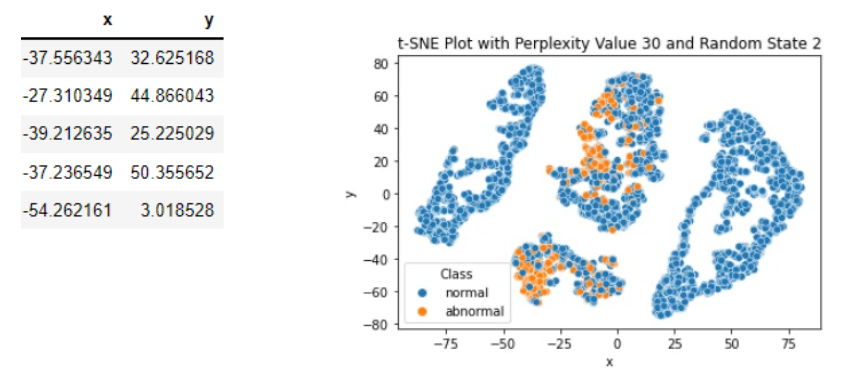
\includegraphics[scale=0.5]{tsne_example_of_output.png}
    \caption{Example of Output}
    \label{}
\end{figure}\end{center}

\subsection{Main Idea of The Algorithm}
\begin{enumerate}
    \item \textbf{\underline{Optimization Problem:}} Given an original high dimensional dataset, we need to solve an optimization for the optimal value of the decision variables that represent the low-dimensional projected coordinates for each observation in the original dataset.\\
    $\vec{x}_i=[x_{1,1},...,x_{1,n}] \Rightarrow \vec{y}_i=[y_{i,1},y_{i,2}],\ i=1,2...,m$.
    \begin{center}\begin{figure}[htbp]
        \centering
        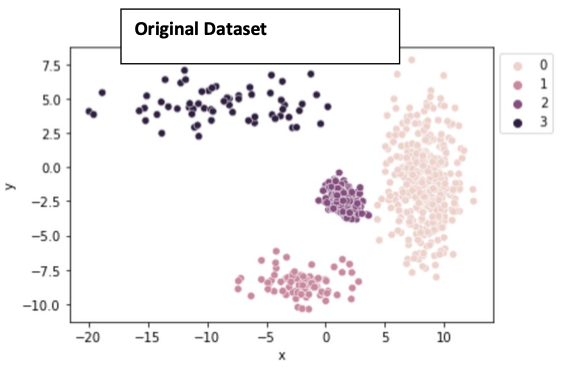
\includegraphics[scale=0.4]{OP_tsne.png}
        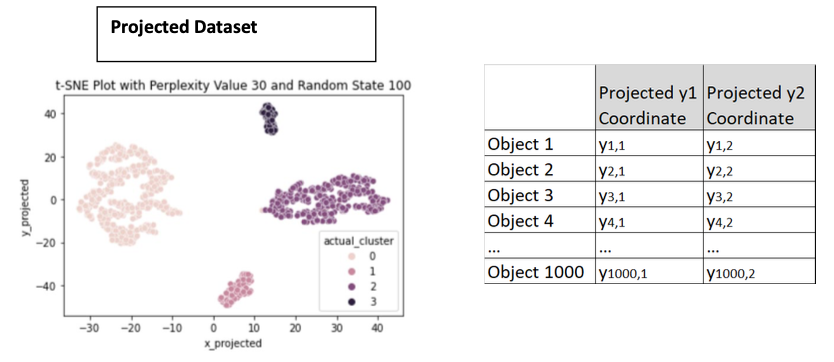
\includegraphics[scale=0.4]{OP_tsne_2.png}
        \caption{Optimization Problem}
        \label{}
    \end{figure}\end{center}
    \item \textbf{\underline{Crates a Similarity matrix $P$ for the Points in the Original Dataset:}}
    Similarity between a given point $\vec{x}_i$ and another point $\vec{x}_j$ is a function of a normal distribution centered at $\vec{x}_i$ with a standard deviation $\sigma_i$ that changes based on the point and how many "neighbors" you think each point in the dataset has. Each entry of the matrix is the \textbf{similarity} between $i$ and $j$.
    \begin{equation}
        \begin{aligned}
        p_{i j}= & \frac{1}{2m}\left(p_{j \mid i}+p_{i \mid j}\right) \\
        & \bullet p_{j \mid i}=\frac{\exp \left(-\frac{\left\|\vec{x}_i-\vec{x}_j\right\|^2}{2 \sigma_i^2}\right)}{\sum_{k \neq i} \exp \left(-\frac{\left\|\vec{x}_i-\vec{x}_k\right\|^2}{2 \sigma_i^2}\right)} \\
        & \bullet p_{i \mid j}=\frac{\exp \left(-\frac{\left\|\vec{x}_i-\vec{x}_j\right\|^2}{2 \sigma_j^2}\right)}{\sum_{k \neq j} \exp \left(-\frac{\left\|\vec{x}_j-\vec{x}_k\right\|^2}{2 \sigma_j^2}\right)}
        \end{aligned}
        \nonumber
    \end{equation}
    \item \textbf{\underline{Creates a Similarity Matrix $Q$ for the Points (i.e., Decision Variables we are Trying to Solve for)} in the \underline{Projected Dataset}:} Similarity between a given point $\vec{y}_i$ and another point $\vec{y}_j$ is a function about $t$-distribution centered at $\vec{y}_i$.
    $$q_{ij}=\frac{(1+\|\vec{y}_i-\vec{y}_j\|^2)^{-1}}{\sum_{k\neq l}(1+\|\vec{y}_k-\vec{y}_j\|^2)^{-1}}$$
    \item Solve the optimization problem:
    \begin{equation}
        \begin{aligned}
            \min_{\{\vec{y}_i\}_{i=1}^m}\textnormal{dist}(P,Q)=D_{KL}(P\| Q)=\sum_i\sum_j p_{ij}\log\frac{p_{ij}}{q_{ij}}
        \end{aligned}
        \nonumber
    \end{equation}
    A heuristic solution to this optimization problem can be found via a \underline{Gradient Descent algorithm}.
\end{enumerate}


Algorithm is heavy on both time and space resources $O(n^2)$. Computationally ineffective for datasets with more than $10000$ observations.

\chapter{Hierarchical Clustering}
\section{Agglomerative and Divisive Hierarchical Clustering Algorithms}
\textbf{Hierarchical clustering algorithms} allow us to display a series of nested clusterings, graphically displayed in a dendrogram.
\begin{center}\begin{figure}[htbp]
    \centering
    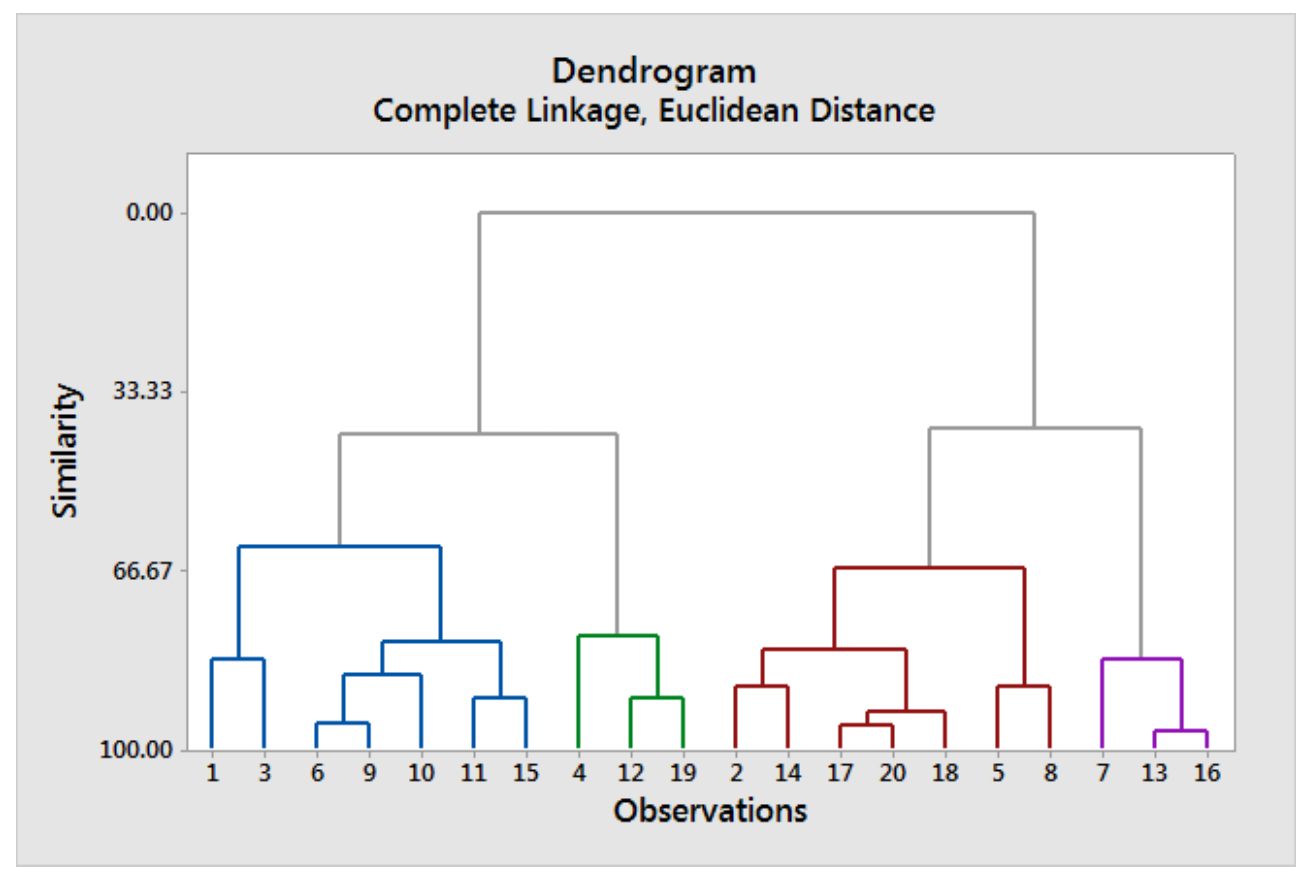
\includegraphics[scale=0.2]{Hierarchical Clustering.png}
    \caption{Hierarchical Clustering Example}
    \label{}
\end{figure}\end{center}

\begin{enumerate}
    \item An \textbf{\underline{ agglomerative hierarchical clustering algorithm}} starts with all objects \textbf{apart in singleton clusters} and then iteratively joins clusters together until all objects
    are in the same cluster.
    \item A \textbf{\underline{ divisive hierarchical clustering algorithm}} starts with all objects \textbf{together} and then iteratively divides clusters together until all objects
    are apart
    in singleton clusters.
\end{enumerate}

\subsection{General Algorithm for Agglomerative Hierarchical Clustering}
\begin{enumerate}[1.]
    \item Create an \textbf{initial proximity matrix of clusters} by calculating the proximity of all objects to each other.
    \begin{center}\begin{figure}[htbp]
        \centering
        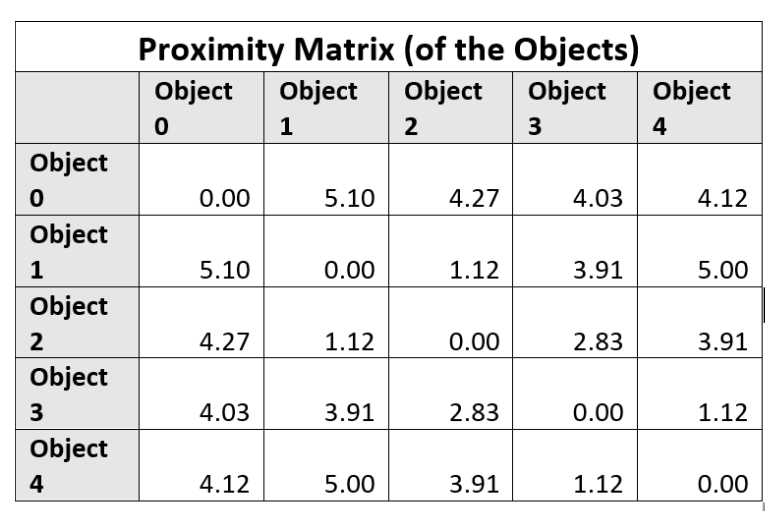
\includegraphics[scale=0.25]{PM.png}
        \caption{Proximity Matrix}
        \label{}
    \end{figure}\end{center}
    \item 
\end{enumerate}

































\end{document}